\chapter{Spójność i spójność drogowa}
\label{ch:topog-spojnosc}

\noindent\textbf{Cel rozdziału.}
Zwartość, badana w rozdziale~07, pozwala wybierać skończone
podpokrycia. Spójność wyraża inne zjawisko: niemożność
podziału przestrzeni na dwa niepuste, rozłączne zbiory otwarte.
Zbadamy jej charakteryzacje, zachowanie przy odwzorowaniach
ciągłych i iloczynach oraz składowe spójne. Następnie
odróżnimy spójność od spójności drogowej i omówimy
spójność lokalną. We wszystkich stwierdzeniach, jeśli
nie zaznaczono inaczej, nie zakładamy aksjomatów oddzielania.

\section{Spójność i jej charakteryzacje}
\label{sec:topog-spojnosc-definicja}

\begin{definicja}[Rozdzielenie i przestrzeń spójna]
\label{def:topog-spojnosc}
Niech $(X,\tau)$ będzie przestrzenią topologiczną.
\emph{Rozdzieleniem} $X$ nazywamy parę $(U,V)$ niepustych,
rozłącznych zbiorów otwartych w $X$ takich, że $X=U\cup V$.
Przestrzeń $X$ jest \emph{spójna}, jeżeli nie istnieje
jej rozdzielenie. Podzbiór $A\subseteq X$ jest spójny,
gdy jest spójny z topologią podprzestrzeni.
Pusta przestrzeń jest zatem spójna.
\end{definicja}

\begin{twierdzenie}[Charakteryzacje spójności]
\label{thm:topog-spojnosc-charakteryzacje}
Dla przestrzeni topologicznej $X$ następujące warunki
są równoważne:
\begin{enumerate}[label=\textup{(\roman*)}]
\item $X$ jest spójna;
\item jedynymi zbiorami równocześnie otwartymi i domkniętymi
w $X$ są $\varnothing$ i $X$;
\item każde ciągłe odwzorowanie $f:X\to\{0,1\}$,
gdzie $\{0,1\}$ ma topologię dyskretną, jest stałe.
\end{enumerate}
\end{twierdzenie}
\begin{proof}
Jeśli istnieje rozdzielenie $X=U\cup V$, to $U$
jest niepusty i właściwy, otwarty, a także domknięty,
bo $X\setminus U=V$ jest otwarty. Odwrotnie, dla
niepustego właściwego zbioru otwarto-domkniętego $U$
para $(U,X\setminus U)$ jest rozdzieleniem. Dowodzi
to równoważności (i) i (ii).

Jeśli $U$ jest niepustym właściwym zbiorem
otwarto-domkniętym, funkcja $f:X\to\{0,1\}$
równa $0$ na $U$ i $1$ na jego dopełnieniu jest
ciągła: przeciwobrazy obu singletonów są otwarte.
Nie jest stała. I odwrotnie, jeśli $f$ jest ciągła
i niestała, oba przeciwobrazy $f^{-1}(\{0\})$,
$f^{-1}(\{1\})$ są niepuste oraz otwarte,
a wzajemnie się dopełniają. Uzyskaliśmy
rozdzielenie $X$. Dla $X=\varnothing$ wszystkie
trzy warunki zachodzą.
\end{proof}

\begin{przyklad}[Przestrzenie dyskretne i niedyskretne]
\label{ex:topog-spojnosc-pierwsze}
Przestrzeń z topologią antydyskretną
$\{\varnothing,X\}$ jest spójna: nie ma niepustego
właściwego zbioru otwartego. Z kolei przestrzeń
dyskretna o co najmniej dwóch punktach nie jest
spójna, ponieważ każdy singleton jest
otwarto-domknięty. Jednopunktowa przestrzeń
jest spójna niezależnie od topologii.
\end{przyklad}

\begin{przyklad}[Spójność nie oznacza aksjomatu Hausdorffa]
\label{ex:topog-spojnosc-sierpinski}
Przestrzeń Sierpińskiego $X=\{0,1\}$ z topologią
$\{\varnothing,\{1\},X\}$ jest spójna: jej jedyne
zbiory otwarto-domknięte to $\varnothing$ i $X$.
Jednocześnie nie jest przestrzenią $T_1$, a tym
bardziej Hausdorffa (por. rozdział~05).
\end{przyklad}

\begin{twierdzenie}[Spójność przedziałów]
\label{thm:topog-spojnosc-przedzialy}
Każdy przedział $I\subseteq\R$, z topologią
indukowaną przez topologię euklidesową, jest
spójny. Odwrotnie, każdy spójny podzbiór
$A\subseteq\R$ jest przedziałem, przy czym
dopuszczamy przedział pusty i jednopunktowy.
\end{twierdzenie}
\begin{proof}
Najpierw niech $a<b$. Przypuśćmy, że $[a,b]$
ma rozdzielenie $U\cup V$. Wybierzmy $u\in U$
i $v\in V$; po ewentualnej zamianie nazw
możemy przyjąć $u<v$. W zbiorze $[u,v]$
rozważmy $S=U\cap[u,v]$ i liczbę $c=\sup S$.
Istnienie kresu wynika z niepustości $S$ i
ograniczenia go z góry przez $v$.
Zbiór $U$ jest względnie domknięty w $[a,b]$,
bo $V=[a,b]\setminus U$ jest względnie otwarty.
Wobec tego $c\in U$: istotnie, z definicji
kresu istnieją elementy $S$ dowolnie bliskie $c$,
a $U$ zawiera swoje punkty domknięcia w $[a,b]$.
Jeżeli $c<v$, względna otwartość $U$ daje
punkt $s\in U$ z $c<s<v$, wbrew definicji $c$.
Jeżeli $c=v$, otrzymujemy $v\in U\cap V$, również
sprzeczność. Zatem $[a,b]$ jest spójny.
Przedział jednopunktowy lub pusty jest spójny
bezpośrednio z definicji.

Niech teraz $I$ będzie dowolnym przedziałem.
Gdyby $I=U\cup V$ było rozdzieleniem,
wybralibyśmy $u\in U$, $v\in V$; ponieważ
$I$ jest przedziałem, cały odcinek $[u,v]$
(z końcami w dowolnej kolejności) zawierałby
się w $I$. Ograniczenia $U\cap[u,v]$ i
$V\cap[u,v]$ rozdzielałyby ten odcinek,
wbrew pierwszej części dowodu.

Odwrotnie, jeśli $A\subseteq\R$ nie jest
przedziałem, istnieją $a,b\in A$ oraz
$c\notin A$ takie, że $a<c<b$.
Zbiory $A\cap(-\infty,c)$ i $A\cap(c,\infty)$
są wówczas niepuste, rozłączne, otwarte
w $A$ i pokrywają $A$. Zatem $A$ nie jest
spójny.
\end{proof}

\begin{twierdzenie}[Zachowanie spójności przez odwzorowania]
\label{thm:topog-spojnosc-obraz-ciagly}
Niech $X,Y$ będą przestrzeniami topologicznymi,
$f:X\to Y$ odwzorowaniem ciągłym, a $A\subseteq X$
spójnym podzbiorem. Wówczas $f(A)$ jest spójny.
W szczególności spójność jest zachowywana
przez homeomorfizmy oraz odwzorowania ilorazowe
(przy obrazie całej przestrzeni).
\end{twierdzenie}
\begin{proof}
Ograniczenie $f|_A:A\to f(A)$ jest ciągłe
i surjektywne; ciągłość wynika z definicji
topologii podprzestrzeni. Gdyby $f(A)$
miało rozdzielenie $U\cup V$, przeciwobrazy
$(f|_A)^{-1}(U)$ i $(f|_A)^{-1}(V)$
byłyby rozłączne, otwarte w $A$, niepuste
dzięki surjektywności i pokrywałyby $A$.
To sprzeczne ze spójnością $A$.
Homeomorfizm jest ciągły i surjektywny
na swój obraz, a odwzorowanie ilorazowe
jest, z definicji, ciągłe i surjektywne.
\end{proof}

\begin{wniosek}[Własność wartości pośredniej]
\label{cor:topog-spojnosc-wartosci-posredniej}
Niech $X$ będzie spójną przestrzenią topologiczną,
$f:X\to\R$ funkcją ciągłą, a $x,y\in X$.
Wtedy dla każdej liczby $t$ leżącej pomiędzy
$f(x)$ i $f(y)$ istnieje $z\in X$ takie,
że $f(z)=t$.
\end{wniosek}
\begin{proof}
Z twierdzenia~\ref{thm:topog-spojnosc-obraz-ciagly}
zbiór $f(X)$ jest spójny, a z twierdzenia
\ref{thm:topog-spojnosc-przedzialy} wynika,
że jest przedziałem. Zawiera $f(x)$ oraz
$f(y)$, więc zawiera także każdą liczbę
pomiędzy nimi.
\end{proof}

\begin{wniosek}[Zwartość, spójność i osiąganie wartości]
\label{cor:topog-spojnosc-zwarty-przedzial}
Jeśli $X$ jest niepustą, zwartą i spójną
przestrzenią topologiczną, a $f:X\to\R$
jest ciągła, to istnieją $m,M\in\R$, $m\le M$,
takie, że $f(X)=[m,M]$. Oba kresy są
osiągane przez $f$.
\end{wniosek}
\begin{proof}
Z twierdzenia Weierstrassa z rozdziału~07
wynika istnienie i osiąganie najmniejszej
i największej wartości $m,M$ funkcji $f$.
Na mocy poprzedniego wniosku każda liczba
pomiędzy nimi należy do $f(X)$; z definicji
kresów nic spoza $[m,M]$ nie należy do obrazu.
\end{proof}

\section{Operacje zachowujące spójność}
\label{sec:topog-spojnosc-operacje}

\begin{twierdzenie}[Suma zbiorów spójnych o części wspólnej]
\label{thm:topog-spojnosc-suma}
Niech $X$ będzie przestrzenią topologiczną,
a $(A_i)_{i\in I}$ rodziną niepustych spójnych
podzbiorów $X$. Jeżeli $\bigcap_{i\in I}A_i\ne
\varnothing$, to $\bigcup_{i\in I}A_i$ jest spójny.
Dla $I=\varnothing$ suma jest pusta i zatem spójna.
\end{twierdzenie}
\begin{proof}
Załóżmy $I\ne\varnothing$ i wybierzmy
$p\in\bigcap_{i\in I}A_i$. Gdyby suma
$A=\bigcup_i A_i$ miała rozdzielenie $U\cup V$,
punkt $p$ należałby do jednego z tych zbiorów,
powiedzmy do $U$. Dla każdego $i$ ograniczenia
$U\cap A_i$ i $V\cap A_i$ są otwarte w $A_i$;
ponieważ $A_i$ jest spójny i $p\in U\cap A_i$,
mamy $A_i\subseteq U$. Zatem $A\subseteq U$,
co przeczy niepustości $V$.
\end{proof}

\begin{figure}[htbp]
\centering
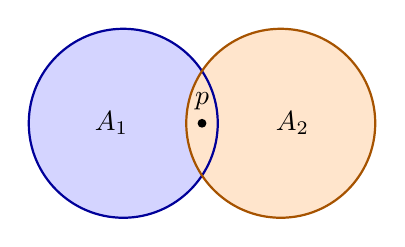
\begin{tikzpicture}[scale=1]
  \fill[blue!17] (-1,0) circle (1.2);
  \fill[orange!20] (1,0) circle (1.2);
  \draw[blue!60!black,thick] (-1,0) circle (1.2);
  \draw[orange!65!black,thick] (1,0) circle (1.2);
  \fill (0,0) circle (1.6pt);
  \node[above] at (0,.05) {$p$};
  \node at (-1.15,0) {$A_1$};
  \node at (1.15,0) {$A_2$};
\end{tikzpicture}
\caption{Dwa zbiory spójne $A_1,A_2$ o niepustej
części wspólnej (z zaznaczonym punktem $p$).
Ich suma jest spójna. Rysunek ilustruje
twierdzenie, nie stanowi jego dowodu.}
\label{fig:topog-spojnosc-suma}
\end{figure}

\begin{twierdzenie}[Domknięcie zbioru spójnego]
\label{thm:topog-spojnosc-domkniecie}
Niech $A\subseteq X$ będzie spójny i niech
$A\subseteq B\subseteq\overline A$, gdzie
domknięcie jest liczone w $X$. Wówczas $B$
jest spójny. W szczególności domknięcie
zbioru spójnego jest spójne.
\end{twierdzenie}
\begin{proof}
Załóżmy, że $B=U\cup V$ jest rozdzieleniem.
Zbiory $U\cap A$, $V\cap A$ są otwarte w $A$
i rozłączne. Co najmniej jeden z nich
jest pusty, ponieważ $A$ jest spójny.
Załóżmy $A\subseteq U$. Wtedy $V$ jest
niepustym zbiorem otwartym w $B$, więc
$V=B\cap W$ dla pewnego otwartego $W\subseteq X$.
Wybierzmy $v\in V$. Ponieważ $v\in\overline A$
i $v\in W$, zachodzi $W\cap A\ne\varnothing$,
a z drugiej strony $W\cap A=V\cap A=\varnothing$,
gdyż $A\subseteq B$. Otrzymujemy sprzeczność.
Przypadek $A\subseteq V$ jest symetryczny.
\end{proof}

\begin{przyklad}[Przecięcie zbiorów spójnych nie musi być spójne]
\label{ex:topog-spojnosc-przeciecie}
Okrąg $S^1=\{(x,y)\in\R^2:x^2+y^2=1\}$
jest spójny: jest ciągłym obrazem odcinka
$[0,2\pi]$ przez $t\mapsto(\cos t,\sin t)$.
Oś pozioma $L=\R\times\{0\}$ jest spójna,
ponieważ jest homeomorficzna z $\R$.
Jednak $S^1\cap L=\{(-1,0),(1,0)\}$
nie jest spójny, gdyż oba singletony są
otwarte w podprzestrzeni dwupunktowej.
\end{przyklad}

\begin{twierdzenie}[Spójność iloczynów]
\label{thm:topog-spojnosc-iloczyn}
Niech $(X_i)_{i\in I}$ będzie rodziną
przestrzeni spójnych. Wówczas iloczyn
$\prod_{i\in I}X_i$ z topologią produktową
jest spójny, także gdy jest pusty.
\end{twierdzenie}
\begin{proof}
Najpierw rozważmy dwie niepuste przestrzenie
spójne $X,Y$. Wybierzmy $y_0\in Y$.
Zbiór $B=X\times\{y_0\}$ jest spójny,
bo jest homeomorficzny z $X$.
Dla każdego $x\in X$ zbiór
$A_x=\{x\}\times Y$ jest spójny,
bo jest homeomorficzny z $Y$, a
$A_x\cap B=\{(x,y_0)\}\ne\varnothing$.
Z twierdzenia~\ref{thm:topog-spojnosc-suma}
wynika, że $A_x\cup B$ jest spójny.
Wszystkie zbiory $A_x\cup B$ zawierają $B$,
więc ich suma $X\times Y$ jest spójna.
Indukcyjnie otrzymujemy spójność dowolnego
skończonego iloczynu niepustych przestrzeni
spójnych; iloczyn pusty jest jednopunktowy.

Niech teraz $X=\prod_{i\in I}X_i$.
Jeżeli $X=\varnothing$, jest spójny z definicji.
W przeciwnym razie ustalmy $p=(p_i)_{i\in I}\in X$.
Dla każdego skończonego $J\subseteq I$
niech $Y_J\subseteq X$ składa się z punktów
$x$, dla których $x_i=p_i$ przy $i\notin J$.
Przestrzeń $Y_J$ jest homeomorficzna ze
skończonym iloczynem $\prod_{i\in J}X_i$,
a więc spójna. Wszystkie $Y_J$ zawierają $p$.
Na mocy twierdzenia o sumie zbiorów spójnych
zbiór $D=\bigcup_{J\subseteq I,\,J\,\text{skończony}}Y_J$
jest spójny.

Wykażmy, że $D$ jest gęsty w $X$.
Niech $W$ będzie niepustym otwartym zbiorem
w $X$. Z definicji topologii produktowej
istnieje punkt $q\in W$ oraz podstawowy
zbiór otwarty $O$ taki, że $q\in O\subseteq W$
i $O=\prod_{i\in I}O_i$, gdzie $O_i=X_i$
poza skończonym zbiorem $J$. Zdefiniujmy
$x_i=q_i$ dla $i\in J$ oraz $x_i=p_i$
dla $i\notin J$. Wówczas $x\in Y_J\cap O$,
więc $W\cap D\ne\varnothing$.
Oznacza to $\overline D=X$, a twierdzenie
\ref{thm:topog-spojnosc-domkniecie}
daje spójność $X$. Nie wybieraliśmy
niezależnie punktów z całej rodziny czynników:
w przypadku niepustego iloczynu jeden punkt
$p$ został już ustalony.
\end{proof}

\begin{uwaga}[Spójność i zwartość iloczynów]
\label{rem:topog-spojnosc-tychonoff}
Twierdzenie~\ref{thm:topog-spojnosc-iloczyn}
nie wymaga twierdzenia Tychonoffa ani
aksjomatu wyboru w dowodzie, gdy iloczyn
jest zadany jako niepusty. Inaczej niż przy
zwartości, wystarczają spójność skończonych
iloczynów i domknięć. Odrębną kwestią jest
wnioskowanie o \emph{niepustości} iloczynu
samych niepustych czynników; w ogólności
wymaga to zasady wyboru.
\end{uwaga}

\section{Składowe spójne i całkowita niespójność}
\label{sec:topog-spojnosc-skladowe}

\begin{definicja}[Składowa spójna]
\label{def:topog-spojnosc-skladowa}
Dla przestrzeni $X$ i punktu $x\in X$
\emph{składową spójną} $C(x)$ nazywamy sumę
wszystkich spójnych podzbiorów $X$
zawierających $x$.
Przestrzeń $X$ jest \emph{całkowicie niespójna},
jeśli wszystkie jej składowe spójne są
jednopunktowe (dla $X=\varnothing$ warunek
jest spełniony).
\end{definicja}

\begin{twierdzenie}[Własności składowych spójnych]
\label{thm:topog-spojnosc-skladowe}
Niech $X$ będzie przestrzenią topologiczną.
Każda składowa spójna jest spójna, domknięta
i maksymalna względem zawierania wśród
spójnych podzbiorów $X$. Dwie składowe
spójne są równe albo rozłączne; w konsekwencji
składowe spójne tworzą rozkład $X$.
Nie muszą być otwarte.
\end{twierdzenie}
\begin{proof}
Dla $x\in X$ rodzina definiująca $C(x)$
jest niepusta, bo zawiera $\{x\}$,
a wszystkie jej elementy mają wspólny punkt
$x$. Twierdzenie~\ref{thm:topog-spojnosc-suma}
daje spójność $C(x)$. Jeśli spójny zbiór
$B$ zawiera $C(x)$, to zawiera również $x$,
więc jest jednym ze zbiorów uczestniczących
w definicji $C(x)$; stąd $B\subseteq C(x)$,
co dowodzi maksymalności.
Domknięcie $\overline{C(x)}$ jest spójne
na mocy twierdzenia
\ref{thm:topog-spojnosc-domkniecie}.
Zawiera $C(x)$, więc z maksymalności
$\overline{C(x)}=C(x)$.

Jeśli $C(x)\cap C(y)\ne\varnothing$, suma
tych dwóch zbiorów jest spójna, a zawiera
$x$ oraz $y$. Z maksymalności obu składowych
wynika $C(x)=C(y)$. Każdy punkt należy do
swojej składowej, więc składowe pokrywają $X$.
\end{proof}

\begin{przyklad}[Składowe nie muszą być otwarte]
\label{ex:topog-spojnosc-Q}
W $\Q$ z topologią podprzestrzeni z $\R$
każdy spójny podzbiór ma co najwyżej jeden
punkt. Istotnie, jeśli zawierałby różne
liczby wymierne $p<q$, to dowolna liczba
niewymierna $r\in(p,q)$ wyznaczałaby
jego rozdzielenie przez przecięcia z
$(-\infty,r)$ i $(r,\infty)$.
Zatem składowymi spójnymi $\Q$ są singletony.
Nie są one otwarte w $\Q$, bo każde
względnie otwarte otoczenie liczby wymiernej
zawiera inne liczby wymierne.
Przestrzeń $\Q$ jest więc całkowicie
niespójna, ale nie dyskretna.
\end{przyklad}

\begin{przyklad}[Zbiór Cantora]
\label{ex:topog-spojnosc-cantor}
Niech $\mathcal C\subseteq[0,1]$ będzie klasycznym
zbiorem Cantora. Jego punkty można jednoznacznie
zapisać jako $x=\sum_{n\ge1}a_n3^{-n}$,
gdzie $a_n\in\{0,2\}$. Dla różnych takich
ciągów pierwsza różna cyfra na pozycji $k$
powoduje różnicę wartości co najmniej
$2\cdot3^{-k}-\sum_{n>k}2\cdot3^{-n}=3^{-k}>0$.
Zatem zapis jest jednoznaczny.

Dla ustalonego skończonego ciągu cyfr
$a_1,\ldots,a_m$ podzbiór punktów o tych
pierwszych $m$ cyfrach jest otwarty
i domknięty w $\mathcal C$. Wynika to z tego,
że punktom odpowiadają ciągi cyfr, a suma
pozostałych wyrazów jest co najwyżej
$\sum_{n>m}2\cdot3^{-n}=3^{-m}$:
zbiory o różnych prefiksach długości $m$
leżą w rozłącznych przedziałach domkniętych
z dodatnimi przerwami i tworzą skończony
rozkład $\mathcal C$. Dwa różne punkty
$\mathcal C$ mają różne cyfry na pewnej pozycji,
więc takie względnie otwarto-domknięte
zbiory je rozdzielają. Każdy spójny podzbiór
$\mathcal C$ zawierający dwa różne punkty
miałby wówczas rozdzielenie. Zatem
$\mathcal C$ jest całkowicie niespójny.

\begin{samepage}
Zbiór Cantora jest zarazem zwarty. Aby to
uzasadnić, dla $m\ge1$ niech
\[
K_m=\bigcup_{(a_1,\ldots,a_m)\in\{0,2\}^m}
\left[\sum_{j=1}^m a_j3^{-j},\,
\sum_{j=1}^m a_j3^{-j}+3^{-m}\right].
\]
\end{samepage}

Każdy $K_m$ jest skończoną sumą
przedziałów domkniętych, a więc jest
domknięty w $\R$. Z reprezentacji cyframi
wynika $\mathcal C\subseteq\bigcap_m K_m$.
Dla inkluzji odwrotnej zauważmy, że zbiory
przedziałów w $K_m$ są zagnieżdżone:
przedział odpowiadający pierwszym $m+1$
cyfrom zawiera się w przedziale wyznaczonym
pierwszymi $m$ cyframi. Dla
$x\in\bigcap_m K_m$ jego położenie
w jednoznacznie wyznaczonym przedziale
$K_m$ dostarcza więc zgodnych ze sobą
prefiksów cyfr $a_1,\ldots,a_m$.
Ponieważ długości tych przedziałów to $3^{-m}$,
otrzymujemy $x=\sum_{n\ge1}a_n3^{-n}$.
Wobec tego $\mathcal C=\bigcap_m K_m$
jest domknięty. Zawiera się w zwartym
przedziale $[0,1]$, zatem jest zwarty
na mocy twierdzenia z rozdziału~07.
\end{przyklad}

\section{Drogi i spójność drogowa}
\label{sec:topog-spojnosc-drogi}

\begin{definicja}[Droga i spójność drogowa]
\label{def:topog-spojnosc-droga}
Niech $X$ będzie przestrzenią topologiczną.
\emph{Drogą} od $x$ do $y$ nazywamy ciągłe
odwzorowanie $\gamma:[0,1]\to X$ takie,
że $\gamma(0)=x$ i $\gamma(1)=y$.
Przestrzeń $X$ jest \emph{spójna drogowo},
jeśli dla każdych $x,y\in X$ istnieje
droga od $x$ do $y$.
\end{definicja}

\begin{uwaga}[Droga a łuk]
\label{rem:topog-spojnosc-luk}
W literaturze nazwy \emph{spójność drogowa}
i \emph{spójność łukowa} bywają używane
zamiennie. Aby uniknąć niejednoznaczności,
tu słowem \emph{droga} określamy dowolne
odwzorowanie ciągłe $[0,1]\to X$;
nie wymagamy jego różnowartościowości.
\emph{Łukiem} będziemy nazywać odwzorowanie
homeomorficzne $[0,1]$ na swój obraz.
Twierdzenia niniejszej sekcji dotyczą dróg.
\end{uwaga}

\begin{lemat}[Odwracanie i składanie dróg]
\label{lem:topog-spojnosc-skladanie-drog}
Jeśli istnieją drogi od $x$ do $y$ oraz
od $y$ do $z$, to istnieje droga od $x$
do $z$. Każda droga od $x$ do $y$ daje
także drogę od $y$ do $x$.
\end{lemat}
\begin{proof}
Jeśli $\gamma$ jest drogą od $x$ do $y$,
to $t\mapsto\gamma(1-t)$ jest drogą od
$y$ do $x$, gdyż $t\mapsto1-t$ jest ciągła.
Jeśli $\delta$ jest drogą od $y$ do $z$,
określmy
\[
\eta(t)=\begin{cases}
\gamma(2t),&0\le t\le\tfrac12,\\
\delta(2t-1),&\tfrac12\le t\le1.
\end{cases}
\]
Obie części są ciągłe na swoich przedziałach,
a w $t=\tfrac12$ ich wartości są równe $y$.
Z lematu o sklejaniu odwzorowań ciągłych
(rozdział~03) wynika ciągłość $\eta$.
Ponadto $\eta(0)=x$, $\eta(1)=z$.
\end{proof}

\begin{twierdzenie}[Spójność drogowa implikuje spójność]
\label{thm:topog-spojnosc-droga-implikuje}
Każda przestrzeń spójna drogowo jest spójna.
Każdy ciągły obraz przestrzeni spójnej
drogowo jest spójny drogowo.
\end{twierdzenie}
\begin{proof}
Niech $X$ będzie spójna drogowo.
Gdyby istniało rozdzielenie $X=U\cup V$,
wybralibyśmy $x\in U$, $y\in V$ i drogę
$\gamma:[0,1]\to X$ od $x$ do $y$.
Odcinek $[0,1]$ jest spójny z twierdzenia
\ref{thm:topog-spojnosc-przedzialy}, a jego
obraz $\gamma([0,1])$ jest spójny z twierdzenia
\ref{thm:topog-spojnosc-obraz-ciagly}.
Przecina jednak oba zbiory $U,V$,
więc ich przecięcia z obrazem rozdzielałyby
ten obraz, co daje sprzeczność.

Jeżeli $f:X\to Y$ jest ciągła i $X$
spójna drogowo, to dla dowolnych
$a,b\in f(X)$ możemy wybrać
$x,y\in X$ z $f(x)=a$, $f(y)=b$.
Droga $\gamma$ od $x$ do $y$ daje
ciągłą drogę $f\circ\gamma$ od $a$
do $b$ w $f(X)$.
\end{proof}

\begin{przyklad}[Zbiory wypukłe]
\label{ex:topog-spojnosc-wypukle}
Każdy niepusty zbiór wypukły $C$ w
przestrzeni unormowanej jest spójny drogowo.
Dla $x,y\in C$ droga
$\gamma(t)=(1-t)x+ty$, $0\le t\le1$,
przyjmuje wartości w $C$ z wypukłości
i jest ciągła, ponieważ działania liniowe
są ciągłe w przestrzeni unormowanej.
W szczególności kule, odcinki i całe
przestrzenie unormowane są spójne drogowo.
\end{przyklad}

\begin{definicja}[Składowa drogowa]
\label{def:topog-spojnosc-skladowa-drogowa}
Dla $x\in X$ \emph{składową drogową} $P(x)$
nazywamy zbiór wszystkich punktów $y\in X$,
które można połączyć drogą z $x$.
\end{definicja}

\begin{stwierdzenie}[Rozkład na składowe drogowe]
\label{prop:topog-spojnosc-skladowe-drogowe}
Dla dowolnej przestrzeni $X$ składowe drogowe
tworzą rozkład $X$. Każda składowa drogowa
jest spójna drogowo i zawiera się w pewnej
składowej spójnej. Nie musi być ani otwarta,
ani domknięta.
\end{stwierdzenie}
\begin{proof}
Zachodzą: zwrotność (droga stała), symetria
(odwrócenie drogi) i przechodniość
(składanie dróg), na mocy lematu
\ref{lem:topog-spojnosc-skladanie-drog}.
Jest to zatem relacja równoważności,
a jej klasy stanowią rozkład $X$.
Jeśli $y,z\in P(x)$, możemy połączyć
$y$ z $x$ i $x$ z $z$; złożenie dróg
pokazuje, że $P(x)$ jest spójna drogowo,
więc i spójna. Dlatego $P(x)\subseteq C(x)$.
Ostatnie zdanie zilustrujemy konkretnym
przykładem poniżej.
\end{proof}

\section{Krzywa sinusowa topologa}
\label{sec:topog-spojnosc-sinus}

\begin{przyklad}[Spójność bez spójności drogowej]
\label{ex:topog-spojnosc-sinus}
Rozważmy podzbiór płaszczyzny
\[
G=\{(x,\sin(1/x)):0<x\le1\},\qquad
T=G\cup(\{0\}\times[-1,1]).
\]
Zbiór $G$ jest spójny drogowo: jest obrazem
przedziału $(0,1]$ przez ciągłe odwzorowanie
$x\mapsto(x,\sin(1/x))$. Mamy także
$T=\overline G$ w $\R^2$. Aby wykazać zawieranie
$\overline G\subseteq T$, zauważmy najpierw,
że z $G\subseteq(0,1]\times[-1,1]$ wynika
$\overline G\subseteq[0,1]\times[-1,1]$.
Jeśli $(x,y)\in\overline G$ i $x>0$, to
w przestrzeni metrycznej $\R^2$ istnieje ciąg
$(x_n,\sin(1/x_n))\in G$ zbieżny do $(x,y)$
(kryterium domknięcia przez ciągi w przestrzeniach
pierwszo przeliczalnych z rozdziału~06). Ponieważ $x_n\to x>0$,
z ciągłości funkcji $t\mapsto\sin(1/t)$
w punkcie $x$ wynika
$y=\lim_n\sin(1/x_n)=\sin(1/x)$, czyli
$(x,y)\in G$. Pozostałe punkty domknięcia
mogą więc należeć jedynie do
$\{0\}\times[-1,1]$.

Odwrotnie, $G\subseteq\overline G$, a każdy
punkt $(0,y)$ odcinka pionowego jest punktem
domknięcia $G$: wybierzmy $\theta\in\R$
z $\sin\theta=y$. Dla dostatecznie dużych $n$
mamy $\theta+2\pi n>0$, liczbę
$(\theta+2\pi n)^{-1}\in(0,1]$ oraz
$\bigl((\theta+2\pi n)^{-1},y\bigr)\in G$;
przy tym pierwsza współrzędna dąży do $0$.
Otrzymujemy $\overline G=T$.
Z twierdzenia~\ref{thm:topog-spojnosc-domkniecie}
wynika, że $T$ jest spójny.

Wykażemy, że \emph{nie istnieje droga w $T$}
łącząca punkt odcinka pionowego z punktem $G$.
Przypuśćmy, że taka droga istnieje.
Po ewentualnym odwróceniu parametrów możemy
przyjąć $\gamma(0)\in\{0\}\times[-1,1]$
oraz $\gamma(1)\in G$.
Zapiszmy $\gamma(t)=(u(t),v(t))$; wtedy
$u(0)=0$, $u(1)>0$, a $u(t)\ge0$.
Niech $t_0$ będzie największym punktem
zbioru $\{t\in[0,1]:u(t)=0\}$.
Istnieje on, ponieważ zbiór ten jest
niepusty i domknięty w $[0,1]$, a zatem
zwarty. Ponieważ $u(1)>0$, mamy $t_0<1$.
Dla $t\in(t_0,1]$ zachodzi $u(t)>0$,
a więc $v(t)=\sin(1/u(t))$.

Z ciągłości $v$ w punkcie $t_0$
wybierzmy $\delta\in(0,1-t_0)$ takie,
że $|v(t)-v(t_0)|<\tfrac12$ dla wszystkich
$t\in[t_0,t_0+\delta]$. Z ciągłości $u$
i nierówności $u(t_0)=0<u(t_0+\delta)$
wynika, na mocy własności wartości pośredniej,
że $u([t_0,t_0+\delta])$ zawiera
$[0,u(t_0+\delta)]$. W tym ostatnim
przedziale znajdują się dodatnie liczby
\[
a_n=(\tfrac\pi2+2\pi n)^{-1},\qquad
b_n=(\tfrac{3\pi}2+2\pi n)^{-1}
\]
dla dostatecznie dużego $n$.
Odpowiadają im czasy $s,t\in(t_0,t_0+\delta]$
takie, że $v(s)=1$ i $v(t)=-1$.
Z nierówności $|v(s)-v(t_0)|<1/2$
i $|v(t)-v(t_0)|<1/2$ otrzymujemy
$2=|v(s)-v(t)|<1$, sprzeczność.
Zatem $T$ jest spójny, ale nie jest
spójny drogowo.

Co więcej, $G$ i $\{0\}\times[-1,1]$
są dwiema składowymi drogowymi $T$:
każdy z nich jest spójny drogowo,
a przed chwilą wykluczyliśmy drogi
między nimi. Składowa drogowa $G$
nie jest domknięta, ponieważ $\overline G=T$.
Odcinek pionowy nie jest otwarty w $T$,
ponieważ każde jego otoczenie w $T$
przecina $G$.
\end{przyklad}

\begin{figure}[htbp]
\centering
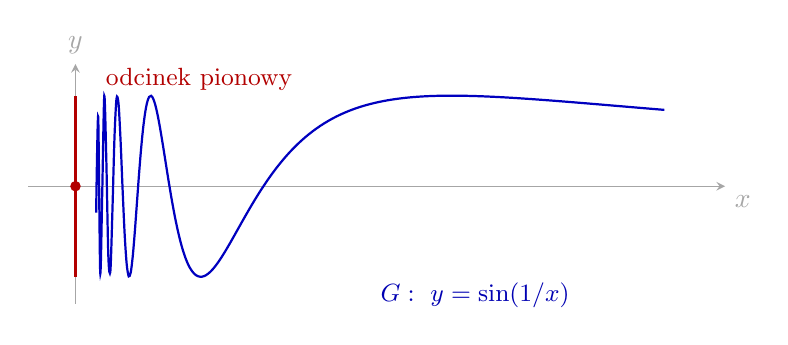
\begin{tikzpicture}[x=7.5cm,y=1.15cm,>=stealth]
  \draw[->,gray!70] (-.08,0)--(1.1,0) node[below right] {$x$};
  \draw[->,gray!70] (0,-1.3)--(0,1.35) node[above] {$y$};
  \draw[red!70!black,very thick] (0,-1)--(0,1);
  \draw[blue!75!black,thick,samples=280,smooth,domain=.035:1]
    plot (\x,{sin(1/\x r)});
  \fill[red!70!black] (0,0) circle (1.9pt);
  \node[anchor=west,red!70!black,font=\small] at (.035,1.18)
    {odcinek pionowy};
  \node[anchor=west,blue!70!black,font=\small] at (.50,-1.2)
    {$G:\ y=\sin(1/x)$};
\end{tikzpicture}
\caption{Krzywa sinusowa topologa $T$: wykres $G$ wraz
z pionowym odcinkiem w $x=0$. Rysunek przedstawia
skończone przybliżenie coraz gęstszych oscylacji,
których nie da się pokonać drogą ciągłą z odcinka
pionowego do wykresu.}
\label{fig:topog-spojnosc-sinus}
\end{figure}
\FloatBarrier

\section{Spójność lokalna}
\label{sec:topog-spojnosc-lokalna}

\begin{definicja}[Spójność lokalna i drogowa lokalna]
\label{def:topog-spojnosc-lokalna}
Przestrzeń $X$ jest \emph{lokalnie spójna},
jeśli dla każdego $x\in X$ i każdego
otwartego otoczenia $U\subseteq X$ punktu $x$
istnieje otwarty spójny zbiór $V$ taki,
że $x\in V\subseteq U$.
Jest \emph{lokalnie spójna drogowo},
jeśli można dodatkowo wymagać, by $V$
był spójny drogowo. Definicje obejmują
przestrzeń pustą.
\end{definicja}

\begin{twierdzenie}[Charakteryzacja spójności lokalnej]
\label{thm:topog-spojnosc-lokalna-komponenty}
Przestrzeń $X$ jest lokalnie spójna wtedy
i tylko wtedy, gdy każda składowa spójna
każdego otwartego zbioru $U\subseteq X$
jest otwarta w $X$.
Analogicznie, $X$ jest lokalnie spójna
drogowo wtedy i tylko wtedy, gdy wszystkie
składowe drogowe wszystkich otwartych
podzbiorów $X$ są otwarte w $X$.
\end{twierdzenie}
\begin{proof}
Przypuśćmy najpierw, że $X$ jest lokalnie
spójna. Ustalmy otwarty $U\subseteq X$
i jego składową spójną $C$ oraz $x\in C$.
Z definicji istnieje otwarty spójny $V_x$
z $x\in V_x\subseteq U$. Ponieważ
$V_x\cap C$ zawiera $x$, twierdzenie
\ref{thm:topog-spojnosc-suma} pokazuje,
że $V_x\cup C$ jest spójny w $U$.
Maksymalność składowej $C$ w $U$ daje
$V_x\subseteq C$. Zatem
$C=\bigcup_{x\in C}V_x$ jest otwarty w $X$.

Odwrotnie, jeśli składowe spójne każdego
otwartego $U$ są otwarte w $X$, to dla
$x\in U$ składowa spójna $C_U(x)$ jest
otwartym spójnym otoczeniem $x$ zawartym
w $U$. Jest to definicja lokalnej spójności.

W wersji drogowej zastępujemy składowe
spójne składowymi drogowymi i stosujemy
lemat~\ref{lem:topog-spojnosc-skladanie-drog}:
dwa spójne drogowo zbiory o niepustej części
wspólnej mają spójną drogowo sumę, ponieważ
drogi można połączyć we wspólnym punkcie.
Pozostały argument jest identyczny.
\end{proof}

\begin{wniosek}[Spójność i drogi w przestrzeni lokalnie drogowej]
\label{cor:topog-spojnosc-lokalna-drogowa}
Jeśli przestrzeń $X$ jest lokalnie spójna
drogowo, to jej składowe drogowe i spójne
są tymi samymi zbiorami. W szczególności,
spójna przestrzeń lokalnie spójna drogowo
jest spójna drogowo.
\end{wniosek}
\begin{proof}
Z poprzedniego twierdzenia każda składowa
drogowa $P$ przestrzeni $X$ jest otwarta
w $X$. Jej dopełnienie jest sumą innych
składowych drogowych, zatem również jest
otwarte. Tak więc $P$ jest otwarto-domknięta.
Jeśli składowa spójna $C$ zawiera $P$,
a także punkt $y\notin P$, to zbiory
$P\cap C$ i $C\setminus P$ byłyby
niepuste, rozłączne, otwarte w $C$
i pokrywałyby $C$. Przeczy to spójności $C$.
Dlatego $C=P$.
\end{proof}

\begin{wniosek}[Spójność zbiorów otwartych w przestrzeni euklidesowej]
\label{cor:topog-spojnosc-euklidesowe}
Niech $n\ge1$ będzie liczbą całkowitą,
a $U\subseteq\R^n$ zbiorem otwartym.
Wówczas $U$ jest spójny wtedy i tylko wtedy,
gdy jest spójny drogowo.
\end{wniosek}
\begin{proof}
Każdy punkt $x\in U$ ma kulę otwartą
$B(x,r)\subseteq U$, a kula jest wypukła,
więc spójna drogowo na mocy przykładu
\ref{ex:topog-spojnosc-wypukle}.
Wynika stąd lokalna spójność drogowa $U$.
Poprzedni wniosek dowodzi implikacji
ze spójności do spójności drogowej,
a implikacja odwrotna wynika z twierdzenia
\ref{thm:topog-spojnosc-droga-implikuje}.
\end{proof}

\begin{przyklad}[Spójność globalna i lokalna to różne własności]
\label{ex:topog-spojnosc-lokalna-przyklady}
Przestrzeń $\R$ jest lokalnie spójna drogowo:
kule otwarte w $\R$ są przedziałami,
a więc są spójne drogowo. Nie jest to
jednak własność wymuszająca spójność
całej przestrzeni: zbiór
$(-2,-1)\cup(1,2)\subseteq\R$ jest lokalnie
spójny drogowo, lecz nie jest spójny.

Z kolei $\Q$ nie jest lokalnie spójny.
Każdy jego spójny podzbiór jest
jednopunktowy (przykład
\ref{ex:topog-spojnosc-Q}), a żaden
singleton nie jest otwarty w $\Q$.
Nie istnieje więc otwarta spójna baza
otoczeń punktu. W szczególności
całkowita niespójność nie wyklucza
lokalnej spójności (przestrzeń dyskretna
jest lokalnie spójna), ale nie gwarantuje jej.
\end{przyklad}

\section{Podsumowanie i kontrprzykłady}
\label{sec:topog-spojnosc-podsumowanie}

\begin{uwaga}[Implikacje i ich ścisłość]
\label{rem:topog-spojnosc-hierarchia}
Spójność drogowa implikuje spójność,
ale implikacja odwrotna jest fałszywa
(przykład~\ref{ex:topog-spojnosc-sinus}).
Lokalna spójność drogowa implikuje lokalną
spójność, ale nie implikuje spójności
globalnej (przykład
\ref{ex:topog-spojnosc-lokalna-przyklady}).
Spójność i zwartość są niezależnymi
własnościami: $\R$ jest spójna,
ale niezwarta; zbiór dwupunktowy z
topologią dyskretną jest zwarty,
ale niespójny. Zamknięty przedział
$[0,1]$ jest zarazem zwarty i spójny.
Spójność nie wymaga aksjomatu $T_2$
(przykład~\ref{ex:topog-spojnosc-sierpinski}).
\end{uwaga}

\begin{uwaga}[Dalsze związki]
\label{rem:topog-spojnosc-dalsze}
Spójność lokalna stanie się istotna
przy badaniu rozmaitości i przestrzeni
nakryciowych. Spójność drogowa pozwala
konstruować klasy dróg i wprowadzać
grupę podstawową, co będzie rozwijane
w topologii algebraicznej. W niniejszym
rozdziale używaliśmy wyłącznie zwykłej
topologii podprzestrzeni, iloczynu,
odwzorowań ciągłych i zwartości
z poprzednich rozdziałów.
\end{uwaga}
